\documentclass{acm_proc_article-sp}

\usepackage{algorithm}
\usepackage[noabbrev]{cleveref}
\usepackage[noend]{algpseudocode}
\usepackage{epstopdf}

\usepackage{framed}

\usepackage{enumitem}

\usepackage{xspace}
\newcommand{\ie}{\emph{i.e.}\xspace}
\newcommand{\eg}{\emph{e.g.}\xspace}
\newcommand{\etal}{\emph{et~al.}\xspace}
\newcommand{\vs}{\emph{v.s.}\xspace}
\newcommand{\rock}{\hbox{\textsc{rocksample}}\xspace}
\newcommand{\poc}{\hbox{\textsc{pocman}}\xspace}
\newcommand{\egreedy}{\hbox{$\varepsilon$-\textsc{greedy}}\xspace}
\newcommand{\eroulette}{\hbox{$\varepsilon$-\textsc{roulette}}\xspace}
\newcommand{\soft}{\hbox{\textsc{softmax}}\xspace}
\newcommand{\rsoft}{\hbox{\textsc{r-softmax}}\xspace}

\newcommand{\RS}[2]{%
\begin{framed}%
\filbreak
	%\noindent
\textbf{Result {#1}:~}{\emph {#2}}%
\end{framed}
}

\begin{document}

\title{Monte Carlo Tree Search Tree Policies}
\subtitle{Randomized Algorithms}
%
% You need the command \numberofauthors to handle the 'placement
% and alignment' of the authors beneath the title.
%
% For aesthetic reasons, we recommend 'three authors at a time'
% i.e. three 'name/affiliation blocks' be placed beneath the title.
%
% NOTE: You are NOT restricted in how many 'rows' of
% "name/affiliations" may appear. We just ask that you restrict
% the number of 'columns' to three.
%
% Because of the available 'opening page real-estate'
% we ask you to refrain from putting more than six authors
% (two rows with three columns) beneath the article title.
% More than six makes the first-page appear very cluttered indeed.
%
% Use the \alignauthor commands to handle the names
% and affiliations for an 'aesthetic maximum' of six authors.
% Add names, affiliations, addresses for
% the seventh etc. author(s) as the argument for the
% \additionalauthors command.
% These 'additional authors' will be output/set for you
% without further effort on your part as the last section in
% the body of your article BEFORE References or any Appendices.

\numberofauthors{2} %  in this sample file, there are a *total*
% of EIGHT authors. SIX appear on the 'first-page' (for formatting
% reasons) and the remaining two appear in the \additionalauthors section.
%
\author{
% You can go ahead and credit any number of authors here,
% e.g. one 'row of three' or two rows (consisting of one row of three
% and a second row of one, two or three).
%
% The command \alignauthor (no curly braces needed) should
% precede each author name, affiliation/snail-mail address and
% e-mail address. Additionally, tag each line of
% affiliation/address with \affaddr, and tag the
% e-mail address with \email.
%
% 1st. author
\alignauthor
Vincent Hellendoorn \\
       \affaddr{4091302}\\
       \affaddr{Msc Computer Science, TU Delft}\\
       \email{v.j.hellendoorn@student.tudelft.nl}
% 2nd. author
\alignauthor
Kaj Oudshoorn \\
       \affaddr{4009444}\\
       \affaddr{Msc Computer Science, TU Delft}\\
       \email{k.oudshoorn-2@student.tudelft.nl}
}

\maketitle

\begin{abstract}
Many intractable problems, like the Travelling Salesman Problem and scheduling problems can be sampled in polynomial time. MCTS uses this fact and applies the intuition of Monte Carlo simulations, by using repeated random samplings. Being the first to ever beat a professional Go player, MCTS is surely a promising research area. Over the years MCTS has improved even further by using so called Tree Policies instead of random sampling. These Tree Policies use a trade-off between exploration and exploitation to determine what to sample during the given timespan. We have evaluated the advantages and disadvantages of a few of these policies (UCB1, \egreedy and \soft) and have used them as building blocks for two novel Tree Policies. 
\end{abstract}

%!TEX root=../report.tex
\section{Introduction}
Many problems are generally intractable due to exponentially large state-spaces. This category of problems includes both classical optimization problems, such as TSP and scheduling problems \cite{browne2012survey}, as well as two-player games such as Go, Chess and 4x4x4 Tic-Tac-Toe \cite{chaslot2010monte, sharma2008knowledge}.
Results from the ML and AI communities indicate that many of these problems, despite having exponential state-spaces, have tractable sample complexity guarantees \cite{sharma2008knowledge}. This is exemplified by the success of AI players in the game Chess (state-space: $2.3 \cdot 10^{49}$ positions) against human opponents, culminating in the defeat of Garry Kasparov by IBM's Deep Blue AI \cite{campbell2002deep}.

Other problems have remained out of the reach of AI approaches for many decades: the two-player game Go is generally considered the last game in which humans consistently outperform computer players, having a state-space of $~2.08 \cdot 10^{170}$ positions on the default board size of 19x19 \cite{tromp2007combinatorics}. However, even on 9x9 boards, where the state-space complexity is lower than that of chess, state-of-the-art AI-approaches failed to outperform human players due to a variety of factors such as a high branching factor \cite{browne2012survey}.

Monte Carlo Tree Search (MCTS) methods were the first to defeat human professionals in Go \cite{coulom2007efficient}, and have come to dominate the Computer Go field \cite{chaslot2010monte}. MCTS (independently proposed in the same year in \cite{coulom2007efficient, kocsis2006bandit, chaslot2006monte}), applies the intuition of Monte Carlo simulations, which work by repeated random sampling, to search trees. Monte Carlo simulations \cite{metropolis1985monte}, in turn, had previously found application in many fields as alternatives to solving mathematically complex problems \cite{liu2008monte}, \eg in evaluating complex integrals with bounded error.

The success of MCTS methods in Go, as well as its general formulation \cite{chaslot2010monte}, have sparked a variety of research into their application to different areas of both optimization problems (with varying succes, \eg \cite{rimmel2011optimization, cazenave2009monte}) and games \cite{schadd2008single, gelly2012grand}.\footnote{See http://www.ualberta.ca/$\sim$szepesva/MCTS/ for a comprehensive overview.} However, in order to be successful, these applications have all but consistently had to replace the (default) UCB1 selection heuristic, which is at the center of the MCTS process. This suggests that the standard approach fails to make optimal use of the structure and information of the search tree.

We propose to investigate a number of alternative tree search heuristics in order to derive properties of the search tree in general and qualities that good heuristics should posses. We evaluate the heuristics on small and large instances of two problems: \rock and \poc (static environment, $10^4 - 10^7$ states \vs dynamic environment, $10^{11} - 10^{18}$ states). These problems fall into the category of games with partially observable state, meaning that in general only a belief about the state of the game is known. We identify four main results:
\vspace{-4mm}
\begin{enumerate}[topsep=0pt,itemsep=-1ex,partopsep=1ex,parsep=1ex]
\item A greedy strategy is poorly equipped when many actions can be chosen.
\item Greater state-spaces necessitate increasingly greedy investigation.
\item ~\soft yields superior performance by connecting the degree of exploration to the total number of simulations.
\item ~\rsoft (our novel variation on \soft) sacrifices little performance in favor of broader applicability to \soft by disregarding the values of rewards used in favor of their ordering.
\end{enumerate}

\section{Monte Carlo Tree Search}

Monte Carlo Tree Search (MCTS) is a heuristic algorithm that is used for online planning. It is easiest explained in relation to games. Take for example a game of chess. The goal is to capture the opponents king while keeping your own king safe. However, in order to obtain that goal a number of moves have to be made by you and your opponent alternatively. Deciding which move to make, given the state of the game, is key to winning the game. Moves can have direct rewards (like the capture of an opponents piece), but in general the effect of a move is only noticed a few turns after it has been made (for example when sacrificing a piece or gaining positional advantages). For this reason it is hard to estimate how good a move is without thinking a few steps ahead. Thinking ahead is, however, considerably hard, given the number of options a player has each turn. At the start of the game, a player can make 20 different moves (sixteen with pawns, four with knights), likewise his opponent also has 20 different moves, resulting in 400 possibilities in the first two moves alone. Without proper knowledge of the values of moves, it is hard to judge which would be the best to play. At the same time, it is infeasible to check all possibilities. 

MCTS solves this problem by only evaluating a selected number of combinations and selecting the move with the highest expected reward. For this purpose MCTS constructs a tree that models the game. In this tree, the root is the starting state, the children are the resulting states of a move and the leafs represent the end state of a game. Each node has a value attached to it, which refers to the expected reward. The tree is constructed by sampling different combinations of actions (paths through the tree). When the leaf node is reached, a reward is obtained which is then propagated back to the root. Every node can update its own expected reward with the obtained value by averaging it over all the obtained rewards. Each tree traversal is called a simulation. In order to make sure the MCTS does not take forever, the amount of simulations is limited. In games where it might take a lot of time to reach an end state, a horizon is added to limit the depth of the traversal.  

%!Tex root=../report.tex

\section{Methodology}

\subsection{Test Data}
We make use of the publicly available framework created by Silver \& Vennes \cite{silver2010monte}. This framework was originally developed to evaluate the performance of MCSTs on games with hidden state, using Partially Observable Monte-Carlo Planning (POMCP). Their framework furthermore contains problem instances for  the POMDP problems \rock and \poc, which form our test set in this research. \\ \\
\rock represents a Mars rover traveling through a grid (sizes 7x8 and 15x15 in our tests), which has to decide whether or not to travel to, and sample from, rocks for reward. The performance depends on the efficiency with which valuables are found. At each step in \rock, 13 actions are available (\eg sampling, moving). \\ \\
\poc is a partially observable variation of Pacman, in which the goal is to collect as many pills possible without getting eaten by the moving ghosts (grid sizes: 7x7 and 17x19). A high reward is reserved for collecting all pills, a penalty is incurred for hitting a wall and dying (the latter causes the game to terminate). The state-space sizes of these problems lies between $10^4$ and $10^8$ positions for \rock, and between $10^{11}$ and $10^{18}$ positions for \poc (due to both the large number of pills and the moving ghosts). At each step, four actions are available in \poc.

\subsection{Tree Policies}
\label{sec:tp}

During the construction of the simulation tree in UCTSearch as in \ref{alg:mcts}, the most important decision to make is the path to traverse. While deciding this at random will certainly give some insight about the structure of the tree (and thus help support the eventual, greedy, selection), this is unlikely to provide good solutions with certainty, particularly when the amount of simulations is small in comparison to the amount of leafs or the state space is large. The Tree Policy adds direction to this search \cite{browne2012survey}. 

A good tree policy strikes a balance between exploration and exploitation. One may argue that visiting nodes that are expected to be useful will help grow confidence in this decision. By sampling different scenario's based around similar decisions, the algorithm gains more knowledge and is able to determine whether these decisions are truly useful or not. But at the same time, there can be actions which do not seem promising at first, but can turn out to be even more rewarding than any other action. This is a trade-off between exploiting promising actions and exploring less-visited actions. Every Tree Policy tries to cope with this trade-off. But while the idea remains the same, their approaches can be quite different. As our objective is to study the quality and properties of various search approaches on MCTS problems, we study a variety of heuristics which are discussed in this section.

\subsubsection{UCB1}
UCB stands for Upper Confidence Bounds. UCB1 is the simplest of the UCB policies proposed by \cite{auer2002finite} and is probably the most well known tree policy in MCTS, together with $\epsilon$-Greedy. For each child node $j$, the importance of visiting that child $Q(j)$ is estimated as follows:
\begin{equation}
Q(j) = \bar{X}_j + c\sqrt{\frac{2 \ln N}{n_j}}
\end{equation}
where $\bar{X}_j$ is the average reward from choosing action $j$, $N$ is the total number of times the root node was visited and $n_j$ is the number of times action $j$ was visited. Hence, the left factor stimulates exploitation (prioritize high-reward actions) and the right hand side stimulates exploration (prioritize relatively little visited actions), where the constant $c$ decides how important exploration is in contrast to exploitation. In our experiments, we defaulted to $c=1$. When this value has been computed for each child, the child with the highest importance will be chosen for the next visit. 

The downside of UCB1 is that there can be occasions where the difference between the highest expected reward and the other rewards is so large that the exploration factor of UCB1 can not bridge the gap. At this point, the formula will behave as if completely greedy, while this may not be the best choice. Even though this problem can be invaded by increasing $c$, this will create a different problem in other parts of the tree where expected rewards are closer together as there UCB1 would only focus on the least visited nodes instead of also slightly favouring promising actions. 

\subsubsection{$\varepsilon$-Greedy}
Another well known method is the \egreedy method\cite{barto1998reinforcement}. In contrast to UCB1, which is deterministic, \egreedy uses randomization in order to achieve some exploration. This policy normally selects the child with the highest expected reward, but with a probability $\varepsilon$ a child is selected at random, uniformly, independent of $\bar{X}_j$. Observing a fair degree of robustness to small changes, in our experiments we used $\varepsilon = 0.2$ (see \Cref{subsec:params}).

This Tree Policy is straightforward, consistently balancing exploration and exploitation in each iteration. Note that it fails to consider that the second or third best actions might be worth exploring more than the worst.

\subsubsection{SoftMax}
\label{subsec:soft}
A different approach of the \egreedy method is \soft\cite{barto1998reinforcement}. The difference is that, instead of switching between exploitation an exploration with a certain probability, \soft starts with a high degree of exploration and steadily becomes more focused on promising areas. This behaviour is achieved by using a variable \emph{temperature} $\tau$. Together with the expected value of each child $j$, the probability $P(j)$ that $j$ is selected to be simulated is calculated as follows:  
\begin{equation}
P(j) = \frac{e^\frac{\bar{X}_j}{\tau}}{\sum_{b=1}^{n} e^\frac{\bar{X}_b}{\tau}}
\end{equation}
When for each child $i$, $\tau \gg \bar{X_i}$, $P(j)$ will be nearly independent of $\bar{X_j}$ and thus the decision of visiting a child will be uniformly distributed. On the other hand, when $\tau$ approaches zero, $P(j)$ will approach 1 if $\bar{X_j}$ is the highest of all children and 0 otherwise. In this sense, \soft is very focused on exploration when temperature is high and becomes more greedy when temperature decreases. The tricky part of \soft is choosing the starting value of $\tau$ how fast $\tau$ decreases. The starting value determines how random your first decisions are and the decrease rate determines how fast you start selecting greedily. 

While \soft fulfills the desire of having a smooth transition of exploration to exploitation, the choice of parameters depends strongly on characteristics of the problem at hand. In particular, as the algorithm must initially be insensitive to any of the rewards, $\tau$ must by necessity be initialized to a value at least as high as the highest reward, if not several times higher. Furthermore, the final value of $\tau$ (typically between 0 and 1) and the type of decrease (linear or exponential) impact the performance as well. Indeed, we found widely varying degrees of performance for seemingly subtle variations in the start and end value of $\tau$. Due to this high need of tuning parameters in \soft, it is not as simple to use as UCB1 or $\epsilon$-Greedy, which may be the reason why it appears to be less popular.

The following two algorithms were constructed following results of our initial evaluation and their rationale is discussed in \Cref{sec:eval}.

\subsubsection{$\varepsilon$-Roulette}
\label{subsec:roulette}
Using the intuition of UCB1, preserving a degree of exploration while favoring high-reward actions, we replaced the random selection method with the ranked roulette selection method. With this selection method, actions are ranked by their performance (with respect to their siblings) and this rank decides the proportion they receive of the roulette wheel. The roulette wheel is "spun" and the appointed action is selected. Arguably this gives an even smaller chance towards actions with a low reward expectation than \egreedy did, but at the same time the second-best action has a better chance to being explored. 

\subsubsection{R-SoftMax}
We furthermore seek to remove the dependency of the temperature parameter in \soft on the problem characteristics. From the calculation of $P(j)$ we can see that there is already a roulette wheel being constructed using the expected rewards of the actions. Rather than using the expected rewards, however, we propose to use their ranks ($r_j$) in comparison to the action values of their siblings. Formula 2 then becomes:
\begin{equation}
P(j) = \frac{e^\frac{r_j}{\tau}}{\sum_{b=1}^{n} e^\frac{n}{\tau}}
\end{equation}



%!Tex root=../report.tex

\begin{figure*}[ht!]
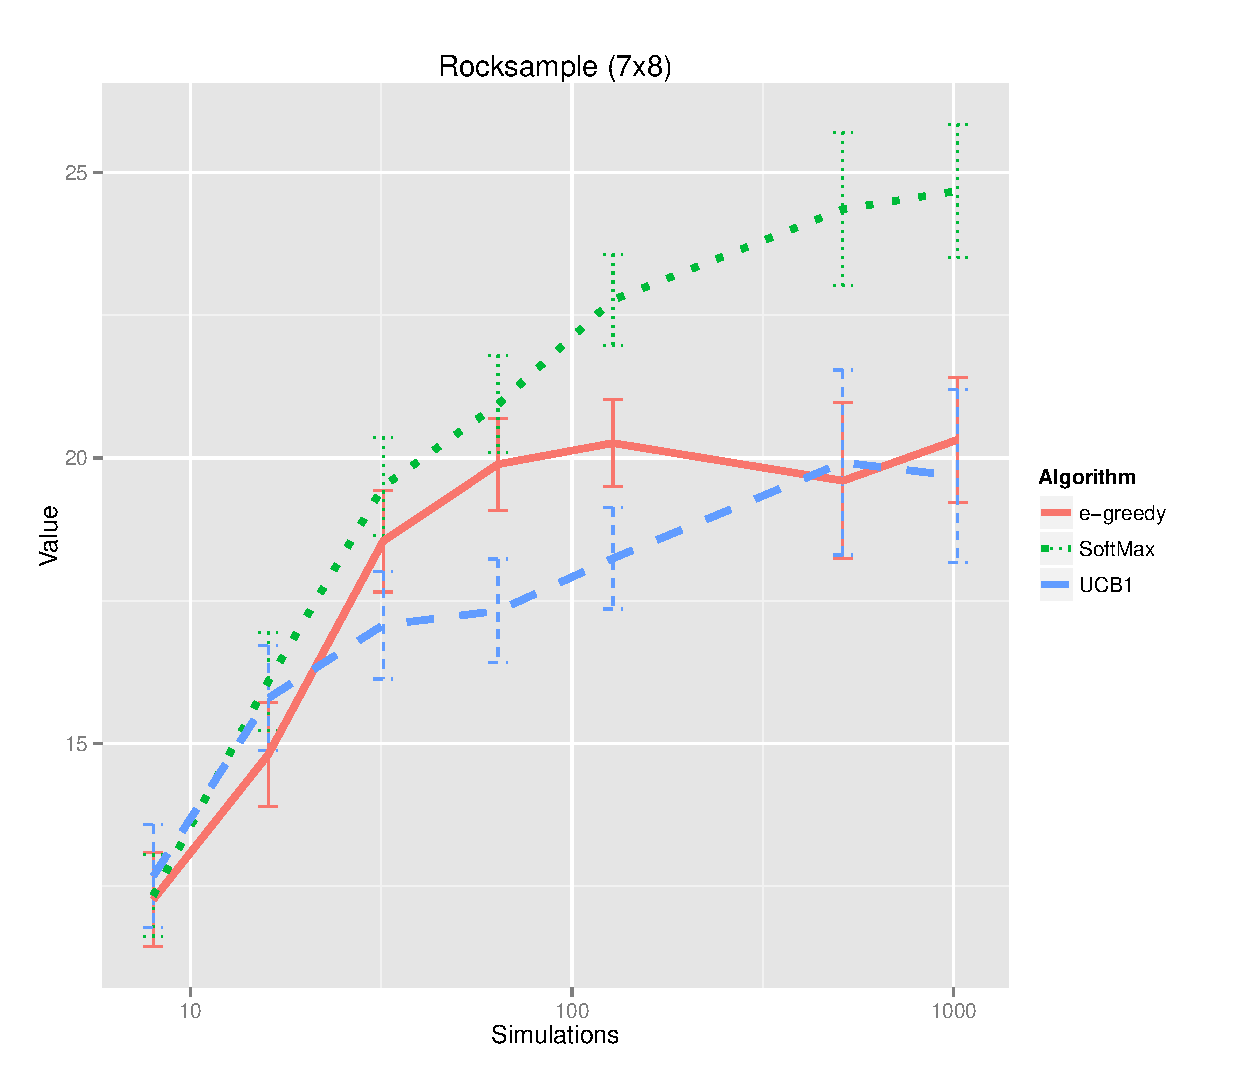
\includegraphics[width=.5\linewidth,height=.3\linewidth]{rocksample78.eps}
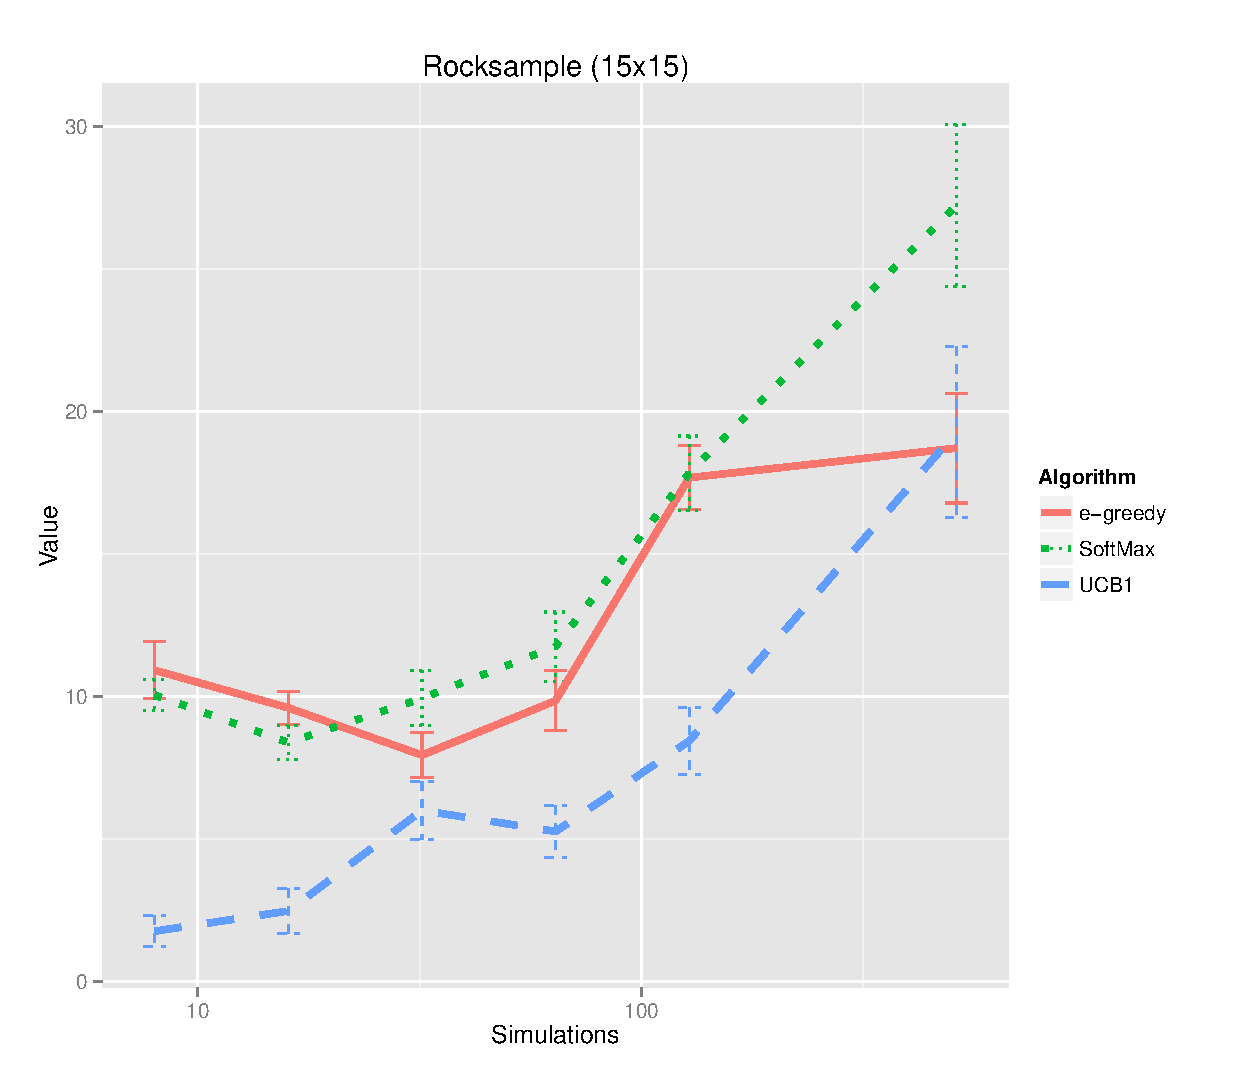
\includegraphics[width=.5\linewidth,height=.3\linewidth]{rocksample1515.eps}
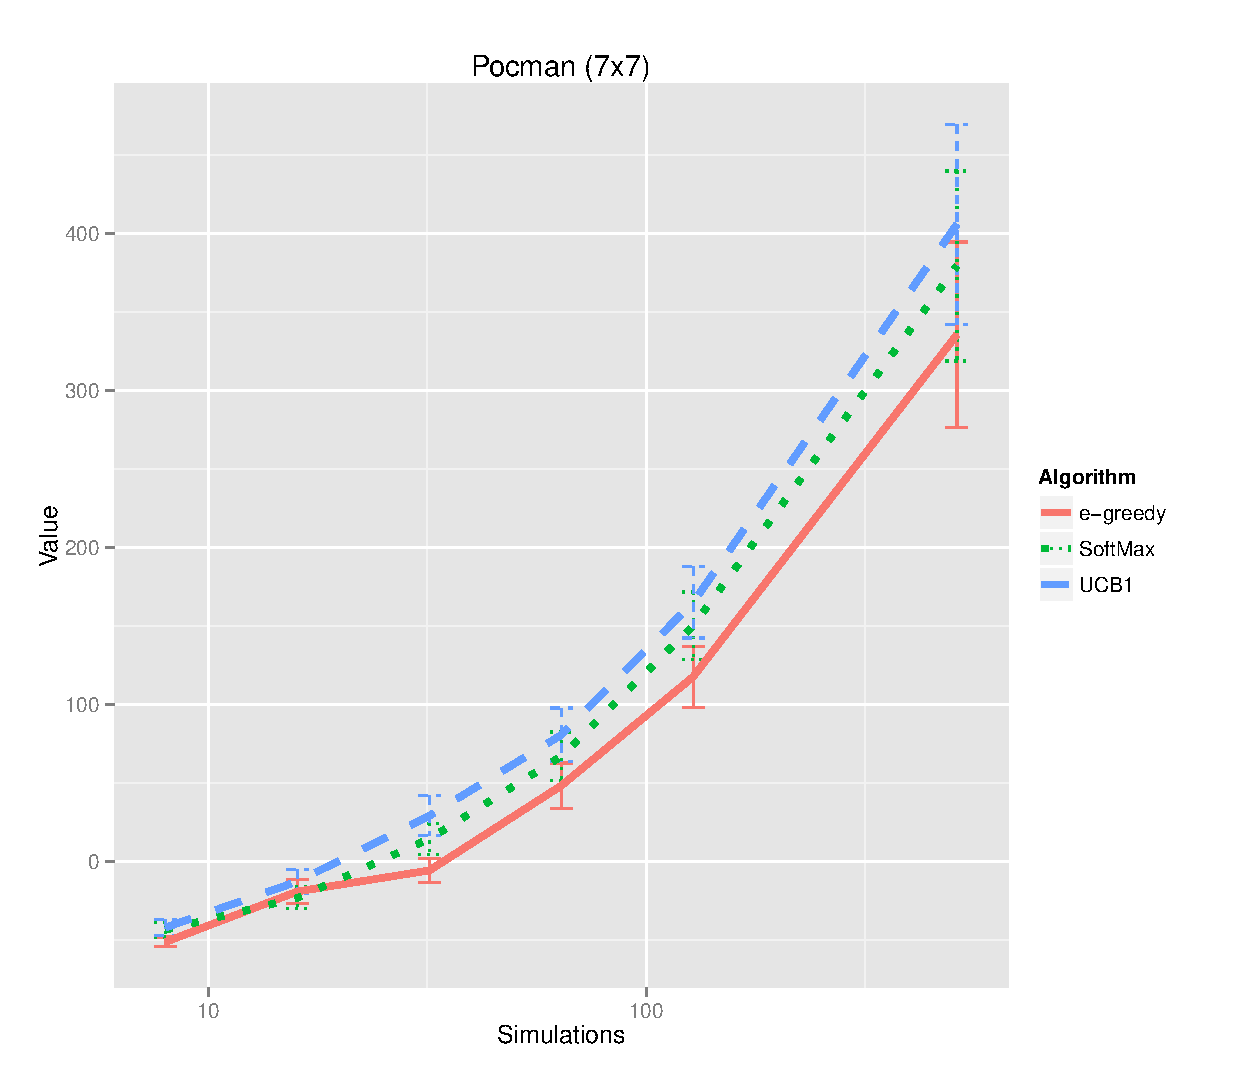
\includegraphics[width=.5\linewidth,height=.3\linewidth]{pocman77.eps}
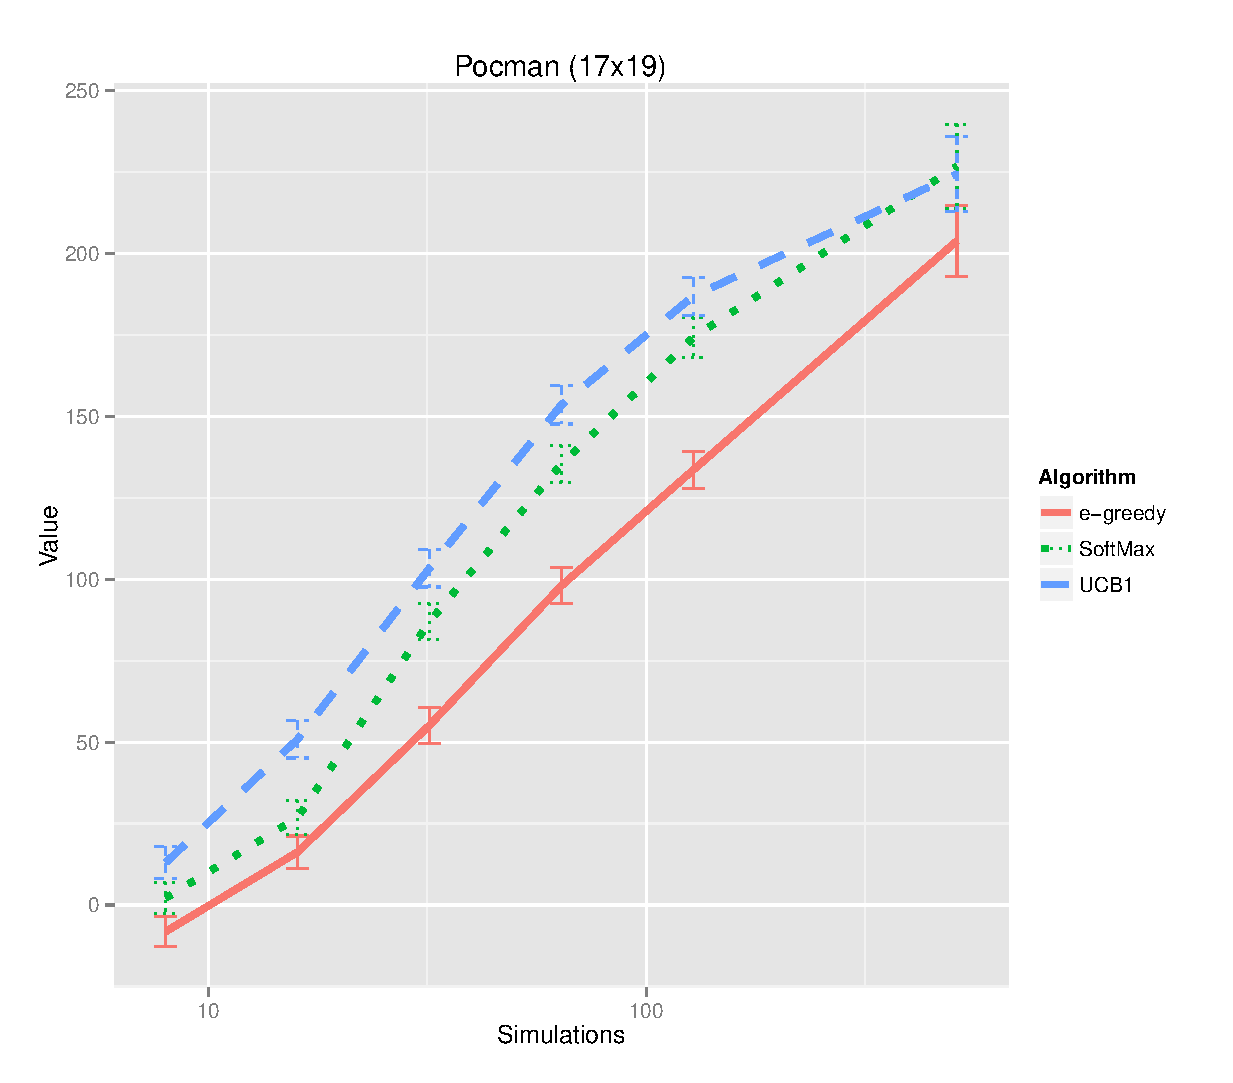
\includegraphics[width=.5\linewidth,height=.3\linewidth]{pocman1719.eps}
\caption{Comparison of UCB1, \soft and \egreedy on two \rock instances and two \poc instances. Note the log-scale on the x-axis, reflecting the increase in simulations. 95\% confidence intervals are indicated on each plot point.}
\label{fig:results1}
\end{figure*}

\section{Evaluation}
\label{sec:eval}
We conduct our analysis of the selected heuristics in three steps, investigating each of the initially studied heuristics separately. Furthermore, to better understand the reason for their relative performance, we propose and evaluate extensions for both \egreedy and \soft. Firstly, we seek to establish whether the default usage of UCB1 is justified on POMDP instances. To this end, we compare UCB1 with two commonly used general-purpose search heuristics: \soft and \egreedy on both the two instances of \rock and of \poc. The results are shown in \Cref{fig:results1}.


\subsection{Performance of UCB1}
As can be seen, performance varies substantially between \rock and \poc. In particular, all algorithms performed comparably on the \poc instances whereas larger gaps in performance were observed on the \rock instances. We identify two probable causes for this discrepancy, which both affect performance of the heuristics: firstly, the number of actions available at every step is much larger in \rock than in \poc (13 \vs 4). The impact of this difference becomes apparent when considering that each simulation recursively chooses an action up to 100 steps ahead. Whereas 256 simulation would suffice to cover all branches up to four steps ahead in \poc, it would only just suffice for two steps in \rock. The second cause lies with the presence of dynamic elements in \poc (ghosts), which may reduce the need to plan far ahead in taking actions.

Both these elements are reflected in the performance of UCB1. Whereas UCB1 is nearly consistently (and often substantially) outperformed on \rock, it achieves top performance (often shared with \soft) on \poc. UCB1 will initially explore all branches but is thereafter more keen to explore branches on which it previously found good performance. This is likely inefficient when many actions are present, as is the case on \rock, as the algorithm may too eagerly give up on an action when one subsequent path leads to poor results. On \poc, however, this strategy works to its advantage, allowing it to explore a few actions in great depth. 

\RS{1}{A greedy strategy is poorly equipped when many actions can be chosen.}

\subsection{Investigating $\varepsilon$-Greedy}
Roughly the inverse of UCB1's performance holds for \egreedy. In particular, \egreedy performs worse than \soft with a greater number of simulations and worse than both other heuristics in the case of a greater state space. This suggests that a constant degree of purely random exploration is inefficient. To evaluate this hypothesis, we propose \eroulette: a variation of \egreedy in which, with probability $\varepsilon$, the action is chosen through roulette wheel sampling based on the expected action value of each child. We compare this variation with \soft in \Cref{fig:results2}. As can be seen, performance improves only on \rock 7x8 and severely decreases on \poc. This suggests that a greater state-space necessitates a shift to increasingly greedy investigation of a few branches towards the end of each iteration. The improved performance on \rock 7x8 furthermore suggests that a greater number of simulations is more efficiently utilized by investigating multiple branches even towards the end of the search.

\RS{2}{Greater state-spaces necessitate increasingly greedy investigation.}

\begin{figure*}[ht!]
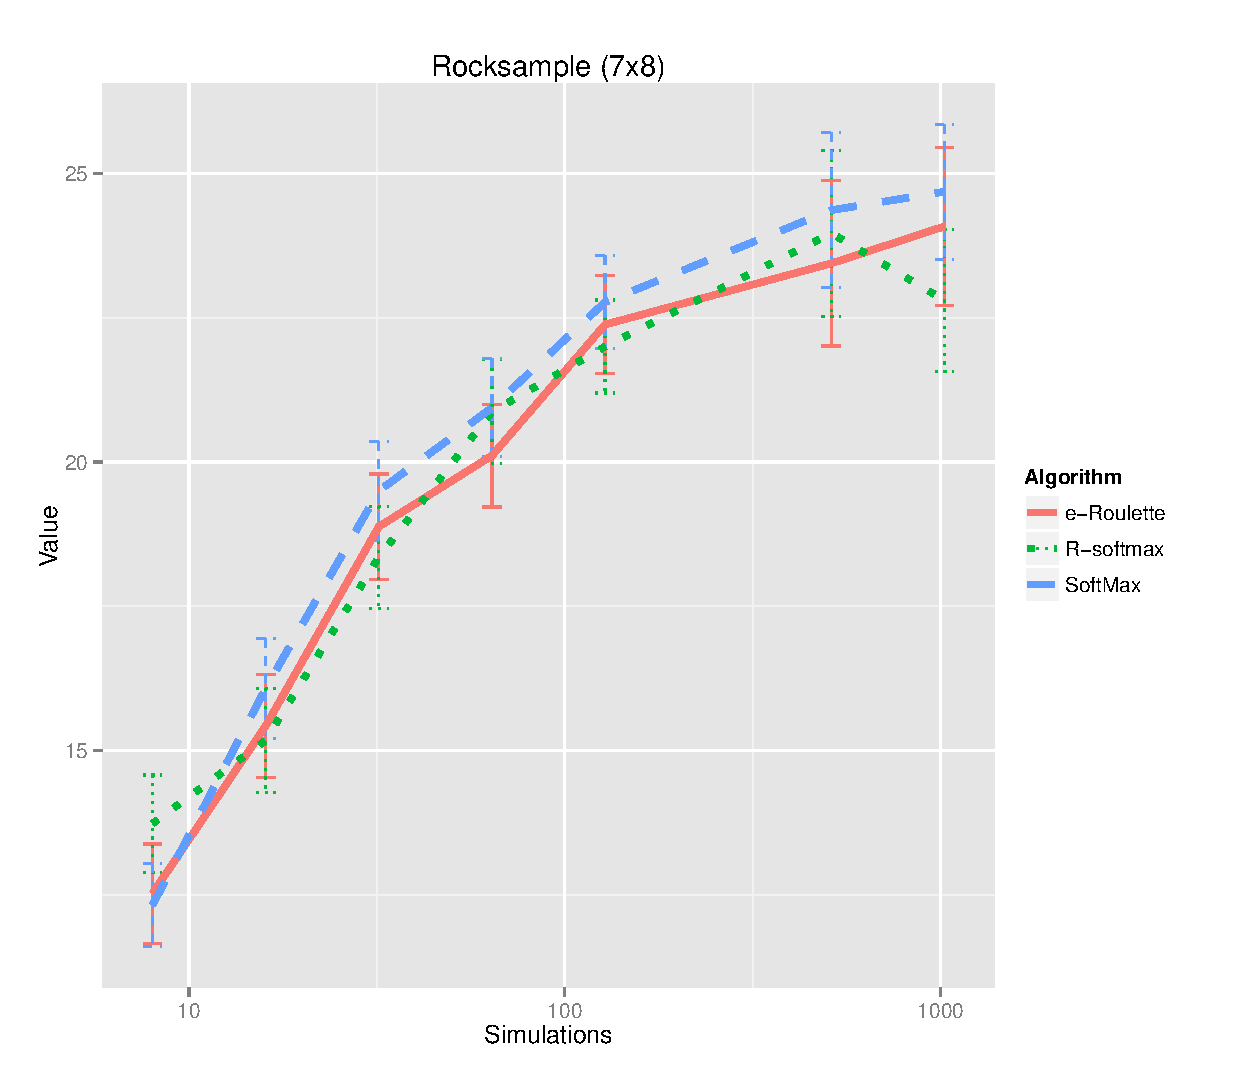
\includegraphics[width=.5\linewidth,height=.29\linewidth]{rocksample78b.eps}
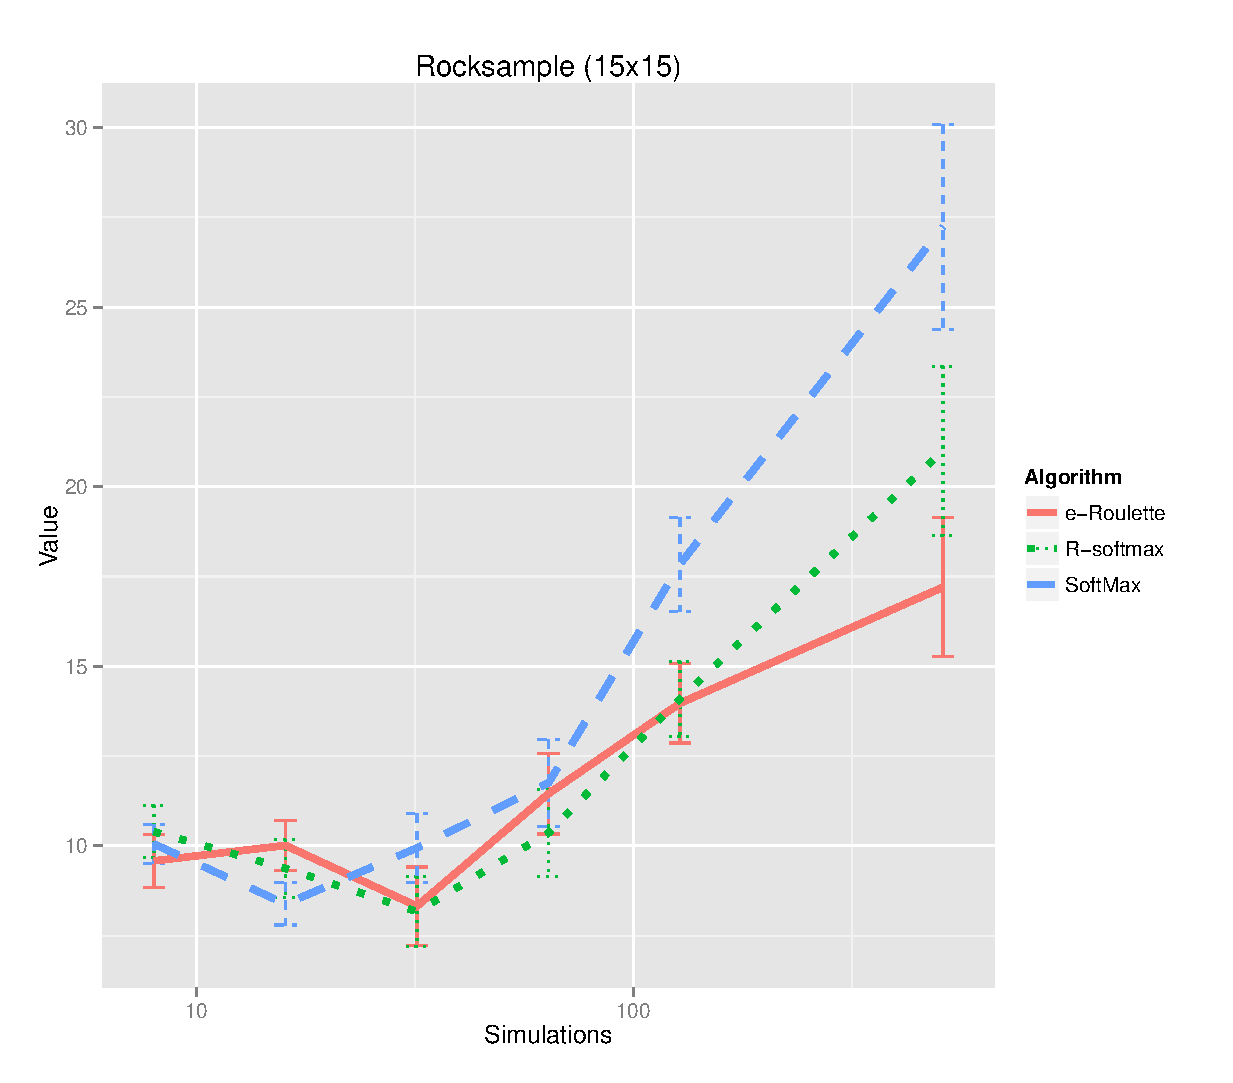
\includegraphics[width=.5\linewidth,height=.29\linewidth]{rocksample1515b.eps}
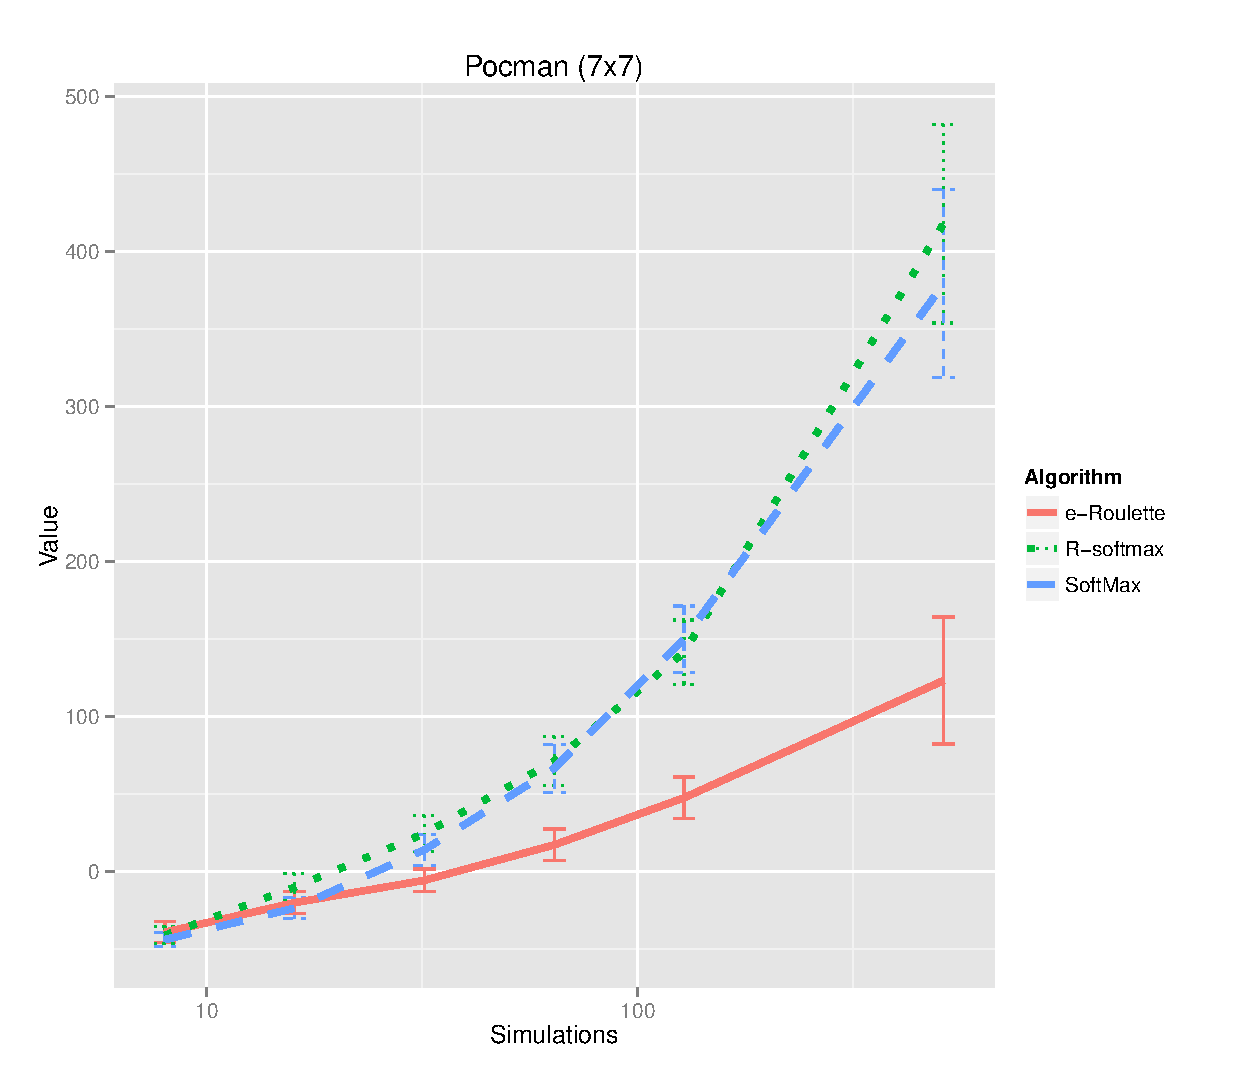
\includegraphics[width=.5\linewidth,height=.29\linewidth]{pocman77b.eps}
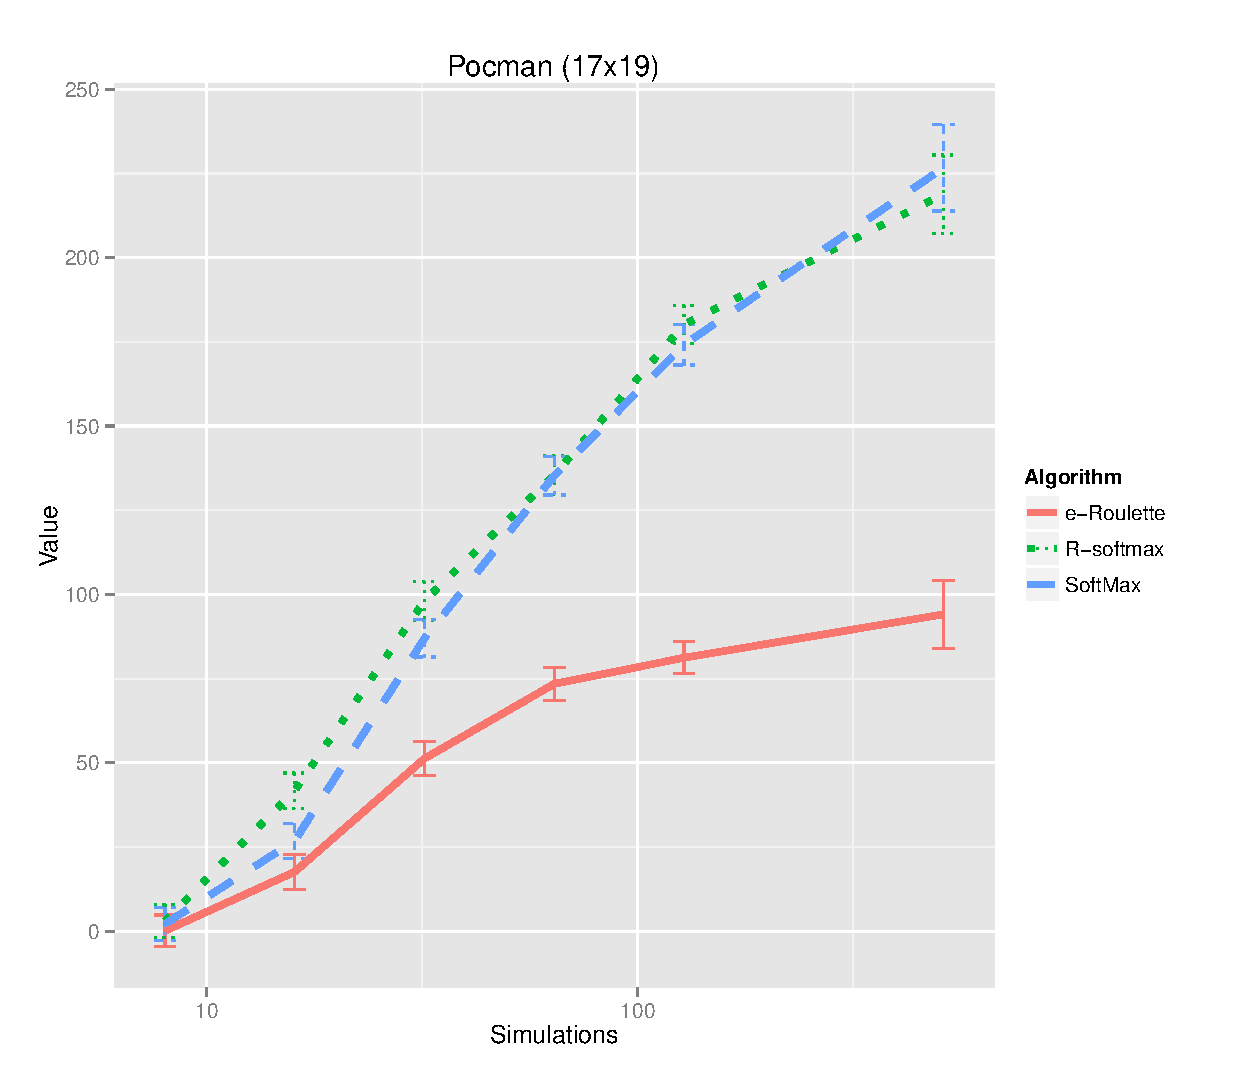
\includegraphics[width=.5\linewidth,height=.29\linewidth]{pocman1719b.eps}
\caption{Comparison of \soft to the two proposed variations: \rsoft and \eroulette, on the two \rock instances and the two \poc instances. Note the log-scale on the x-axis, reflecting the increase in simulations. 95\% confidence intervals are indicated on each plot point.}
\label{fig:results2}
\end{figure*}

\subsection{Investigating SoftMax}
In general, \soft performed best of the tested heuristics. \soft employs a temperature scheme in which the algorithm becomes progressively more greedy as the number of simulations increases. As such, it will initially visit all next actions with roughly equal likelihood and increasingly focus its search on promising branches. Its good performance has strong implications: it suggests that the tree structure can efficiently be exploited by using the relative amount of \emph{information} present at each node (what fraction of simulations were run) to suggest the amount of \emph{randomization} with which decisions should be made.

\RS{3}{\soft yields superior performance by connecting the degree of exploration to the total number of simulations.}

As was noted in \Cref{subsec:soft}, \soft suffers from the need to manually configure the $\tau$ parameter (both start and end value), as well as the rate of decrease of the temperature. We found that this parameter was very sensitive to the actual values of actions that were present in the problem, \eg for \poc a much higher initial value was needed than in \rock as different branches of the search tree yielded widely varying rewards. This strong dependency on the specified rewards for each action adds overhead to the application of this heuristic to a new domain.

We propose a variation to \soft named \rsoft. In this algorithm, we replace each reward with its \emph{rank} in the ordered list of rewards of all children of the current node under consideration. As such, the algorithm is substantially more robust to the absolute rewards chosen. We propose to initialize $\tau$ to the number of distinct actions present, as this will start the algorithm with a high degree of random exploration. We furthermore found that the resulting algorithm is fairly robust with respect to the final value of $\tau$ and suggest setting this to $1/4$. The results are shown in \Cref{fig:results2}. As can be seen, \rsoft almost consistently performs as well as \soft (which was hand-tuned on each instance), with the exception of \rock 15x15. Future work may further investigate extensions.

\RS{4}{\rsoft sacrifices little performance in favor of broader applicability to \soft by disregarding the values of rewards used in favor of their ordering.}


\section{Threats to Validity}
This research constitutes an exploratory study of search heuristics, investigating their relative performance on a relatively small number of problems. As such, the main threats to the validity of the research described in this paper are external, reflecting the degree to which results presented here generalize to other datasets. This concerns the number of different problems investigated, the number of simulations used  and but the values of the parameters for each Tree Policy.

\subsection{Number of problems}
We have run experiments for two different types of problems belonging to the POMDP domain (\rock and \poc) with varying sizes. MCTS, however, has found application in many different domains and it is not unlikely that search trees in some other domains have fundamentally different characteristics. This is even reflected in our own experiments, where we found that \eroulette performed substantially better in \rock than in \poc. To reduce this threat, we have chosen a sample of problems and problem sizes that reflects prior work on POMDPs. Furthermore, \rsoft yielded promising results in an unrelated test following communication with E. Walraven. Further investigation of the evaluated heuristics is needed to evaluate these results on different domains. \\ \\

\subsection{Number of Simulations}
Experiments were performed using a limited number of simulations (8 to 512). These numbers have so far not been enough to show a limit on the performance for each of the Tree Policies. It is therefore unclear how the Tree Policies will behave when the number of simulations (greatly) increases. In particular, we expect some policies to end up deteriorating in performance when executed with a large number of simulations, the same behaviour that can be seen when overfitting occurs in reinforcement learning.

\subsection{Parameters for Tree Policies}
\label{subsec:params}
For the experiments, parameters needed to be chosen for the Tree policies. This concerned in particular \egreedy and \soft. For the former, we chose $\varepsilon$ (the probability of sampling an action at random) to be 0.2, after observing that it was fairly robust with respect to variations in this number. In practice, a number of ML strategies may be used to establish the optimal value for this parameter, which may benefit the performance of \egreedy. The \soft algorithm required tuning of both the start and end values of $\tau$ and the rate of decay. We found that exponential decay yielded substantially superior performance to linear decay. For the values of $\tau$, we hand-tuned the algorithm on each problem instance. Different values of $\tau$ may improve the results for different numbers of simulations as well. Given the already excellent performance of \soft, we deem it unlikely that this substantially influences the overall results.

\section{conclusion}
In this paper we have evaluated a number of Tree Policies that are being used by MCTS in order to solve intractable problems. This evaluation took place in the domains of \rock and \poc: two POMCP problems that are both static and dynamic and have a large amount of states. Most notifiable is that performance is improved when there is a transition between exploration and exploitation during simulations. 

Using this result we have constructed \rsoft: a more domain independent version of \soft. At the minor cost of a slight drop in performance, \rsoft avoids the quirks of parameter tuning, that comes with the usage of \soft. 

As of such we get one step closer towards obtaining a golden Tree Policy that can be used without a lot of knowledge about the domain. Whether this actually holds, can be investigated by looking at more, different domains. Obtaining better performance might be feasible if we look at the ideas that other Tree Policies bring. Taking the amount of times an action has already been visited into account, like UCB1 does, might improve the obtained results. Another option would be to investigate whether one should behave differently depending on how deep you are in the tree, but this is left for future work.

%\section{conclusion}
In this paper we have evaluated a number of Tree Policies that are being used by MCTS in order to solve intractable problems. This evaluation took place in the domains of \rock and \poc: two POMCP problems that are both static and dynamic and have a large amount of states. Most notifiable is that performance is improved when there is a transition between exploration and exploitation during simulations. 

Using this result we have constructed \rsoft: a more domain independent version of \soft. At the minor cost of a slight drop in performance, \rsoft avoids the quirks of parameter tuning, that comes with the usage of \soft. 

As of such we get one step closer towards obtaining a golden Tree Policy that can be used without a lot of knowledge about the domain. Whether this actually holds, can be investigated by looking at more, different domains. Obtaining better performance might be feasible if we look at the ideas that other Tree Policies bring. Taking the amount of times an action has already been visited into account, like UCB1 does, might improve the obtained results. Another option would be to investigate whether one should behave differently depending on how deep you are in the tree, but this is left for future work.

\bibliographystyle{abbrv}
\bibliography{sigproc}  % sigproc.bib is the name of the Bibliography in this case

\end{document}